\subsection{Evaluation method}
We evaluated our method with two different datasets : CREMI and ISBI 2012 datasets.\\
Both are composed of Drosophila adult brain images.\\

A very simple architecture is used for the training.
It's composed of 6 layers of convolution.\\
In~\cite{turaga_maximin_2009}, the original architecture had 4 convolutionnal
layers with 5 features in each. We decided to add more layers and features as
it gave us better results. 
Batch normalisation was also added as it has also given us better results in
our experiments.\\

The architecture is described in detail in table~\ref{tab:archi}. As we can
see, our network takes a 2D image as input whereas both datasets (as we will
detail afterwards) are 3D images. We decided to use 2D images as it was a
simplification of the problem and reduced training time drastically, allowing
us to test our method more effectively.\\
In all of our test, a 3D image of size $X\times Y\times Z$ is considered as $Z$
images of size $X\times Y$ which were stacked together to get back a 3D image.\\

\begin{table}[!htbp]
	\centering
	\begin{tabular}{rllllll}\toprule
		Layer & Kernel & Strides & Features & BN &  Activation & Output shape \\
		\midrule
		Input  &  &  & & & & (21, 21, 1)  \\
		Convolution & (5, 5) & (1, 1) & 8 & Y & ReLU  & (21, 21, 8)  \\
		Convolution & (5, 5) & (1, 1) & 32 & Y & ReLU  & (21, 21, 32)  \\
		Convolution & (5, 5) & (1, 1) & 32 & Y & ReLU  & (21, 21, 32)  \\
		Convolution & (5, 5) & (1, 1) & 32 & Y & ReLU  & (21, 21, 32)  \\
		Convolution & (5, 5) & (1, 1) & 8 & Y & ReLU  & (21, 21, 8)  \\
		Convolution & (5, 5) & (1, 1) & 2 & N & sigmoid  & (21, 21, 2)  \\
		\bottomrule
	\end{tabular}
	\caption{Architecture used in all of our experiments}
	\label{tab:archi}
\end{table}


\subsection{CREMI}
The CREMI (Circuit Reconstruction from Electron Microscopy Images) dataset has three volumes but we decided to use only one (volume A) for our training.
This allows us to use the remaining two for validation and testing.\\
This 3D image has a size of 1250x1250x125. Its corresponding grountruth was also provided in the dataset. 
The segmentation constitutes of labeled connected components with really thin
edges, we can see an example in figure~\ref{fig:cremi_example}.\\
Having labeled connected components instead of borders was really helpful for
our training since we need to know if two pixels belong to the same object,
which was pretty straightforward with this format.\\
For the evaluation, we used the CREMI library that was given with the dataset
in Python 2. We, then, adapted it in Python 3 as to use it more efficiently
with our existing codebase.\\

\begin{figure}[!htbp]
    \centering
    \begin{subfigure}[t]{0.45\textwidth}
        \centering
        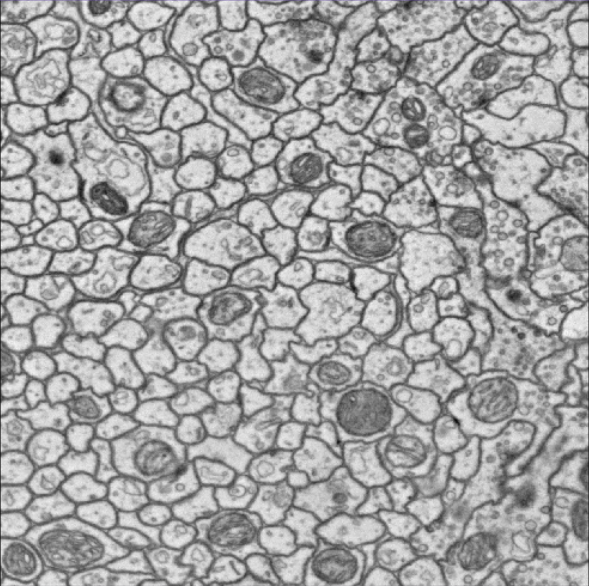
\includegraphics[height=0.6\textwidth]{./images/cremi_orig_1.png}
        \caption{Original image}
    \end{subfigure}%
    ~ 
    \begin{subfigure}[t]{0.45\textwidth}
        \centering
        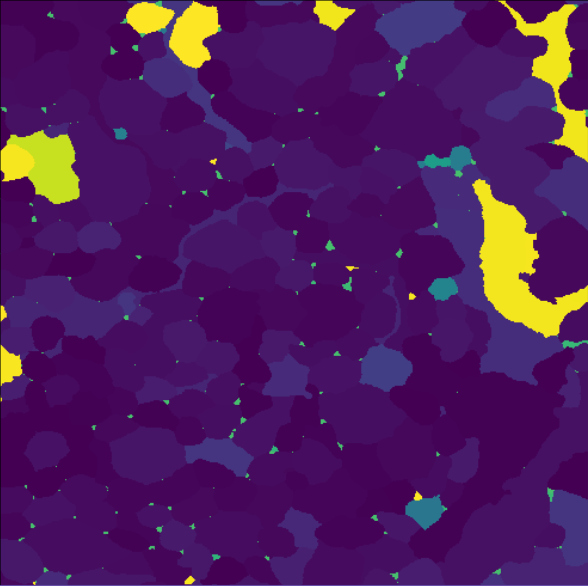
\includegraphics[height=0.6\textwidth]{./images/cremi_gt_1.png}
        \caption{Groundtruth}
    \end{subfigure}
    \caption{CREMI dataset (volume A)}
	\label{fig:cremi_example}
\end{figure}

Once our model is trained a question arises : how to get an image segmentation from the affinity graph ?\\
The affinities were averaged/weighted in~\cite{turaga_maximin_2009} but other
methods could also work.\\

We used two different methods to answer this problem.\\
First of all, a BPT (Binary Partition Tree) of our affinity graph and then a
graph cut could be a first idea, which is a bit more complex than just
averaging the affinities. 

However, even with a strong threshold for our cut (around 0.99), isthmus appeared and fused two different objects together.
This is heavily penalized by the Rand Index and not a desirable outcome.\\
An other method, that got rid of isthmus, was to average the affinities and
then threshold the result, which we used in all of our testing as it was the best solution
(relative to the BPT + graph cut).\\
An illustration of the isthmus issue can be seen in
figure~\ref{fig:cremi_isthmus} .


\begin{figure}[!htbp]
	\centering
	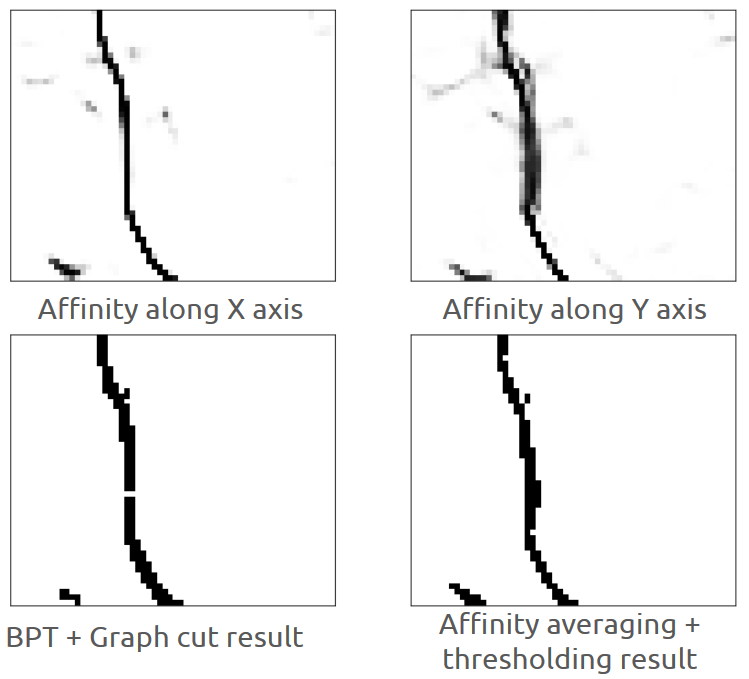
\includegraphics[width=0.7\linewidth]{./images/cremi_isthmus.png}
	\caption{Illustration of the isthmus issue in our segmentation}%
	\label{fig:cremi_isthmus}
\end{figure}

\begin{figure}[!htbp]
    \centering
    \begin{subfigure}[t]{0.31\textwidth}
        \centering
        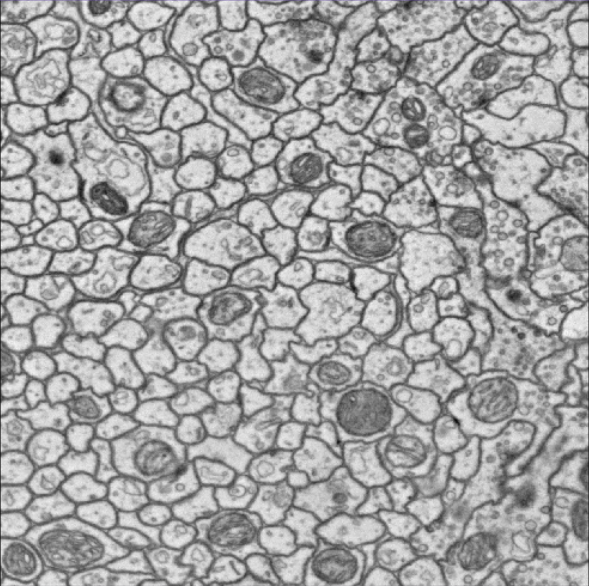
\includegraphics[height=0.7\textwidth]{./images/cremi_orig_1.png}
        \caption{Original image}
    \end{subfigure}%
    \begin{subfigure}[t]{0.31\textwidth}
        \centering
        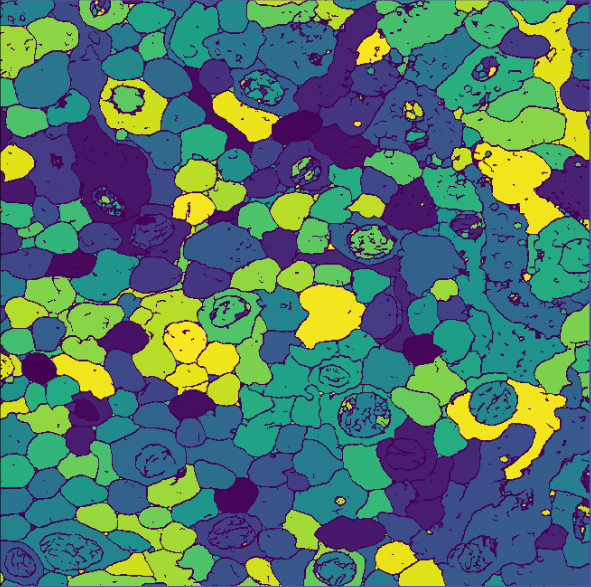
\includegraphics[height=0.7\textwidth]{./images/cremi_out_1.png}
        \caption{Our segmentation}
    \end{subfigure}%
    \begin{subfigure}[t]{0.31\textwidth}
        \centering
        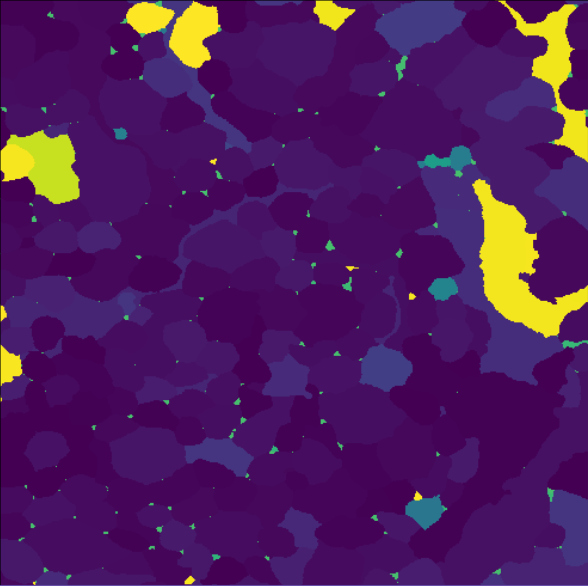
\includegraphics[height=0.7\textwidth]{./images/cremi_gt_1.png}
        \caption{Groundtruth}
    \end{subfigure}
	\caption{Results on the CREMI dataset volume A (Training set)}
	\label{fig:cremi_results_a}
\end{figure}

Our results are promising as the different objects are well segmented, as
illustrated in figure~\ref{fig:cremi_results_a}. 
However we can see that the nuclei are not well segmented as they should be
part of the cell. This is a logical issue since on a local scale, it is hard to
differentiate between the border of a nucleus and the border of a cell.\\

\begin{figure}[!htbp]
    \centering
    \begin{subfigure}[t]{0.31\textwidth}
        \centering
        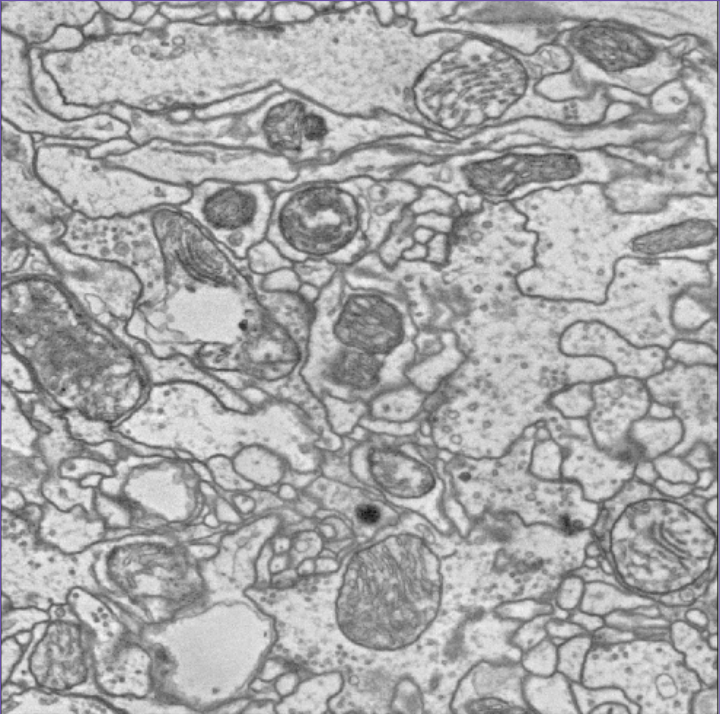
\includegraphics[height=0.7\textwidth]{./images/cremi_orig_2.png}
        \caption{Original image}
    \end{subfigure}%
    ~ 
    \begin{subfigure}[t]{0.31\textwidth}
        \centering
        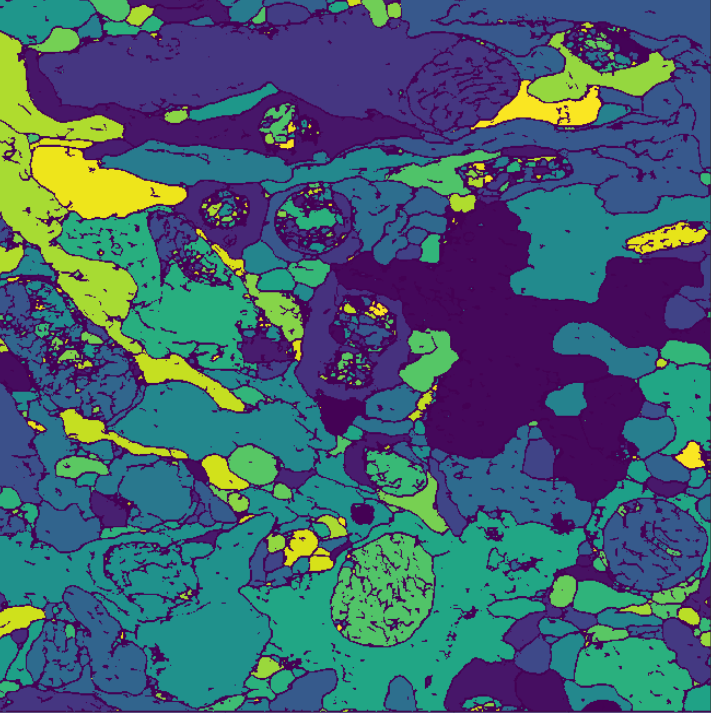
\includegraphics[height=0.7\textwidth]{./images/cremi_out_2.png}
        \caption{Our segmentation}
    \end{subfigure}
    ~ 
    \begin{subfigure}[t]{0.31\textwidth}
        \centering
        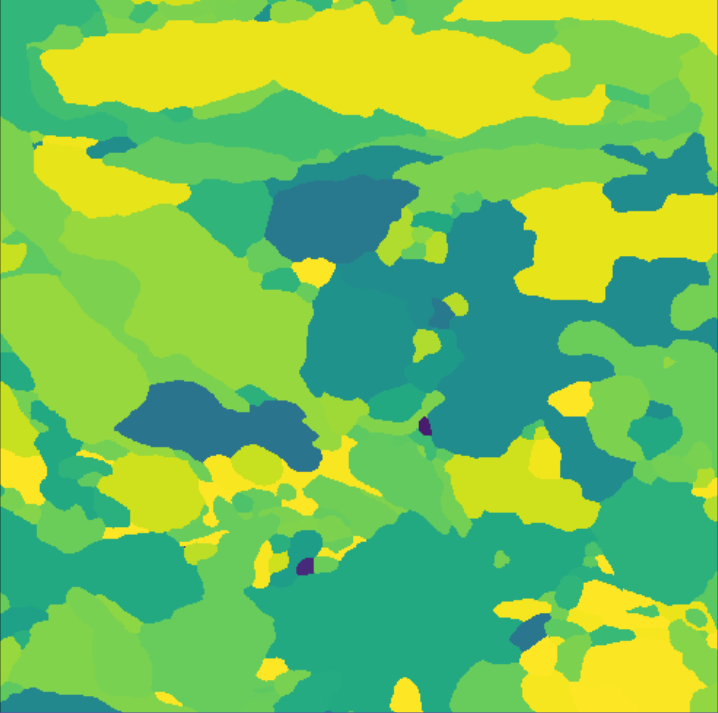
\includegraphics[height=0.7\textwidth]{./images/cremi_gt_2.png}
        \caption{Groundtruth}
    \end{subfigure}
	\caption{Results on the CREMI dataset volume B (Test set)}
	\label{fig:cremi_results_b}
\end{figure}

The second volume (volume B) was used as the test set.
The image was similar to the one in the first volume but the objects are more
"stretched out."\\
As we can see in figure~\ref{fig:cremi_results_b} the objects are well
segmented but we had the same issues as on our training set.\\
The segmentation is obviously a bit worse since we dind't train on this image,
but they are still encouraging.\\

To get a better understanding of our results, we can evaluate the segmentation, 
according to the Rand index and the VOI (variation of information) merge and split.\\ 
The Rand index should be the highest as possible, closer to 1 and VOI should be lower to be better.\\
In this example, we evaluated on all slices of our 3D images and averaged the
final result.\\

\begin{table}[!htbp]
	\centering
	\begin{tabular}{|c|c|c|c|}
		\hline
		& Rand index & \thead{VOI merge \\(lower is better)} & \thead{VOI split\\(lower is better)} \\
		\hline
		\makecell{MALIS : Training set \\(original architecture)} & 0.53 & 2.08 & 1.32\\
		\hline
		MALIS : Training set & 0.61 & 1.25 & 1.03\\
		\hline
		MALIS : Test set & 0.53 & 1.57 & 1.38\\
		\hline
	\end{tabular}
	\caption{Results on the CREMI dataset}
\label{tab:cremi_res}
\end{table}

As we can see in table~\ref{tab:cremi_res}, in the original architecture of 4 layers, 
the Rand index is 0.53 while we got 0.61 with our training set and 0.53 with our test set.
We achievied better results than the original architecture with our small
improvements, but it will be hard to improve them much more with the current
method.\\

Thus, our results are hopeful knowing the architecture used was really simple.\\ 
Our results are still far from the state of the art but it could get even
better by improving various parts of the methos, as we will detail later.\\

\subsection{ISBI 2012}

We also evaluated our method on the ISBI 2012 Challenge dataset
which is composed of a single $512\times512\times30$ image of drosophilia brain
image.\\

\begin{figure}[!htbp]
    \centering
	\begin{subfigure}[t]{0.31\textwidth}
        \centering
        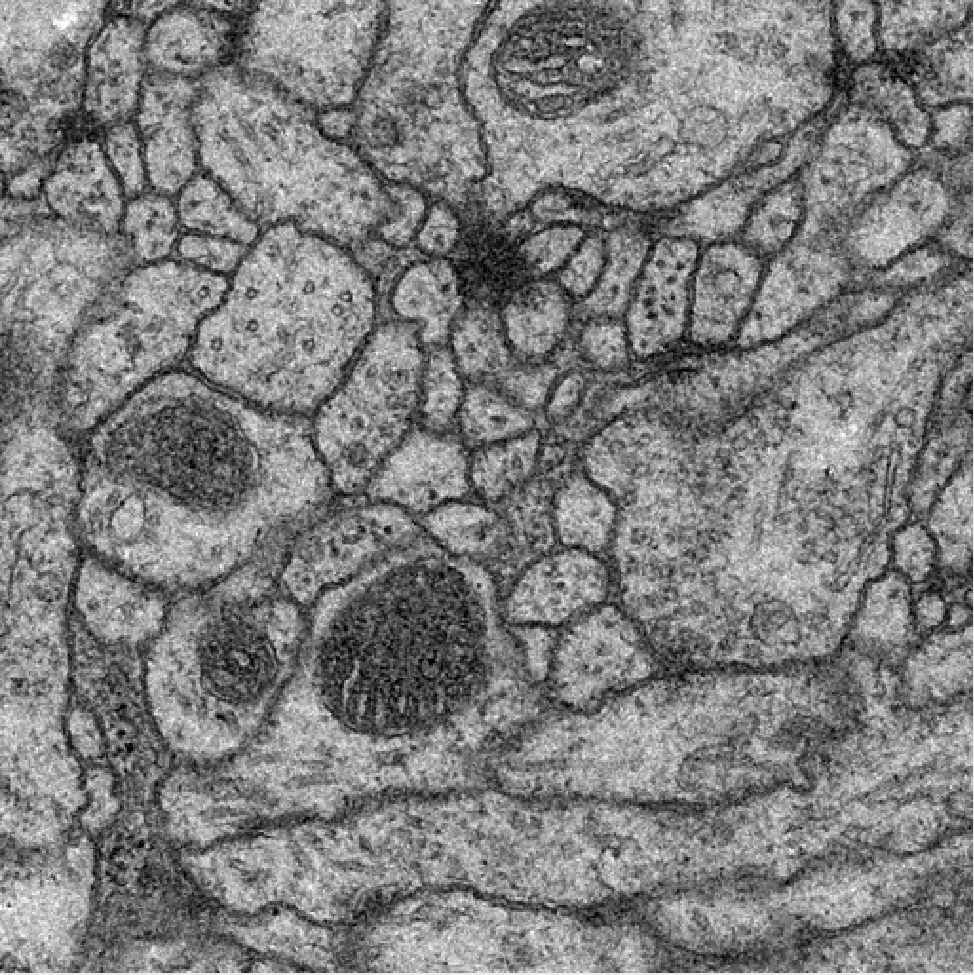
\includegraphics[height=0.7\textwidth]{./images/isbi_orig_1.png}
        \caption{Original image}
    \end{subfigure}%
    \begin{subfigure}[t]{0.31\textwidth}
        \centering
        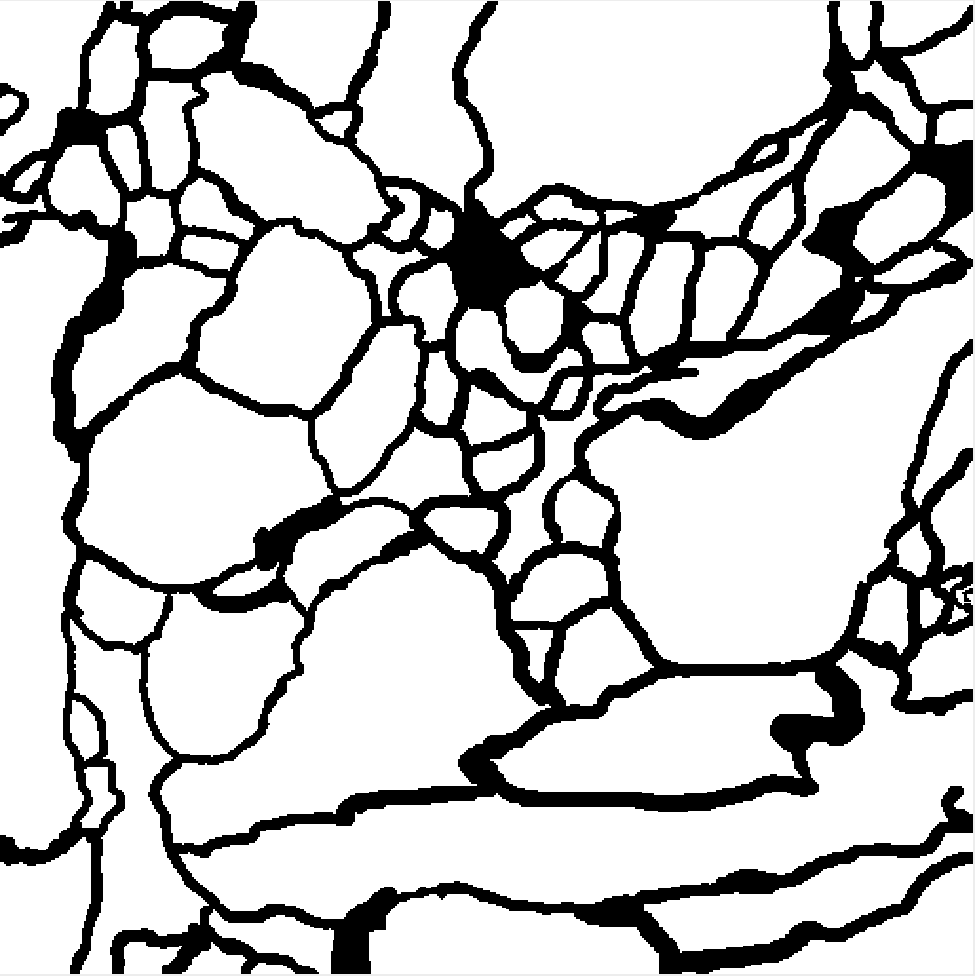
\includegraphics[height=0.7\textwidth]{./images/isbi_gt_1.png}
        \caption{Groundtruth}
    \end{subfigure}
    \caption{ISBI dataset example}
	\label{fig:isbi_example}
\end{figure}

The groundtruth provided with the dataset is composed of borders in black and
cells in white, which we then computed the labeled connected components of as pre
processing for our trainig.
The test set was given with no groundtruth (as it is a challenge) and we had to
submit our output to the challenge's leaderboard to get our scores.
We evaluated using FIJI (Fiji Is Just Imagej) on the training set as an evaluation script was given
for it in the challenge.\\

The same architecture that we used for the CREMI dataset was used for the ISBI dataset.\\

\begin{figure}[!htbp]
    \centering
    \begin{subfigure}[t]{0.31\textwidth}
        \centering
        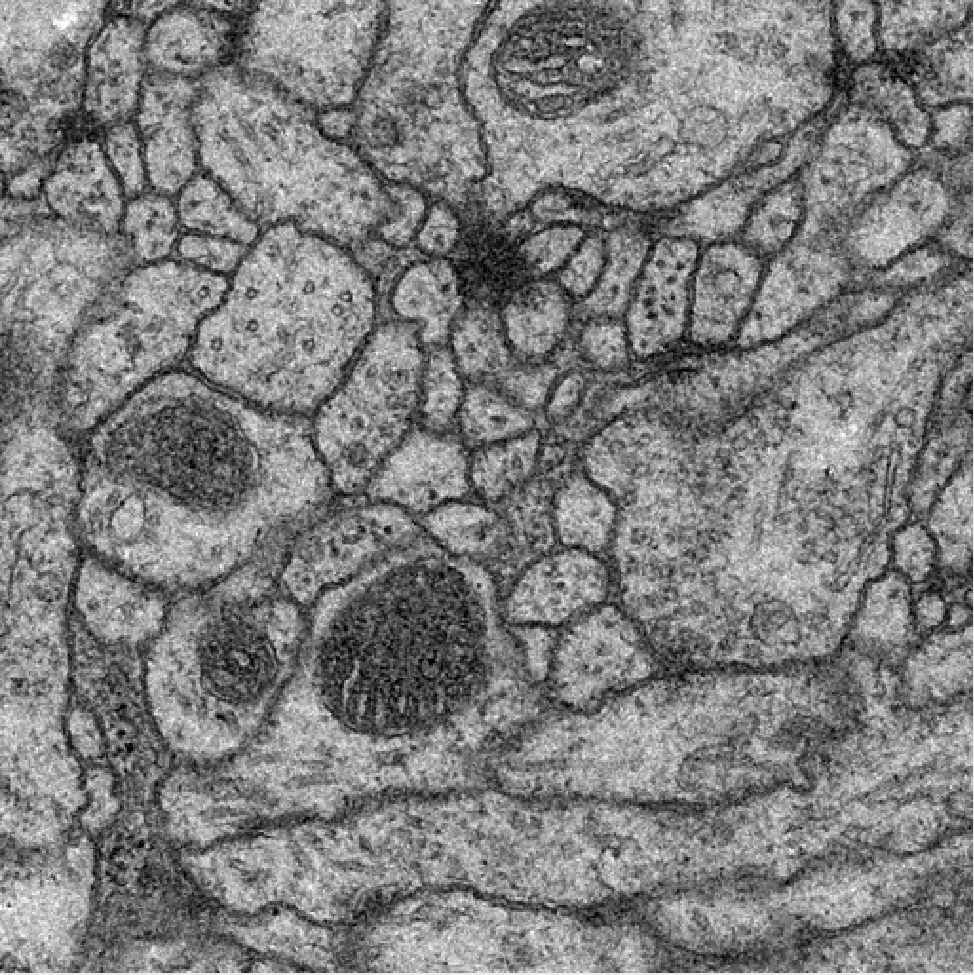
\includegraphics[height=0.7\textwidth]{./images/isbi_orig_1.png}
        \caption{Original image}
    \end{subfigure}%
    \begin{subfigure}[t]{0.31\textwidth}
        \centering
        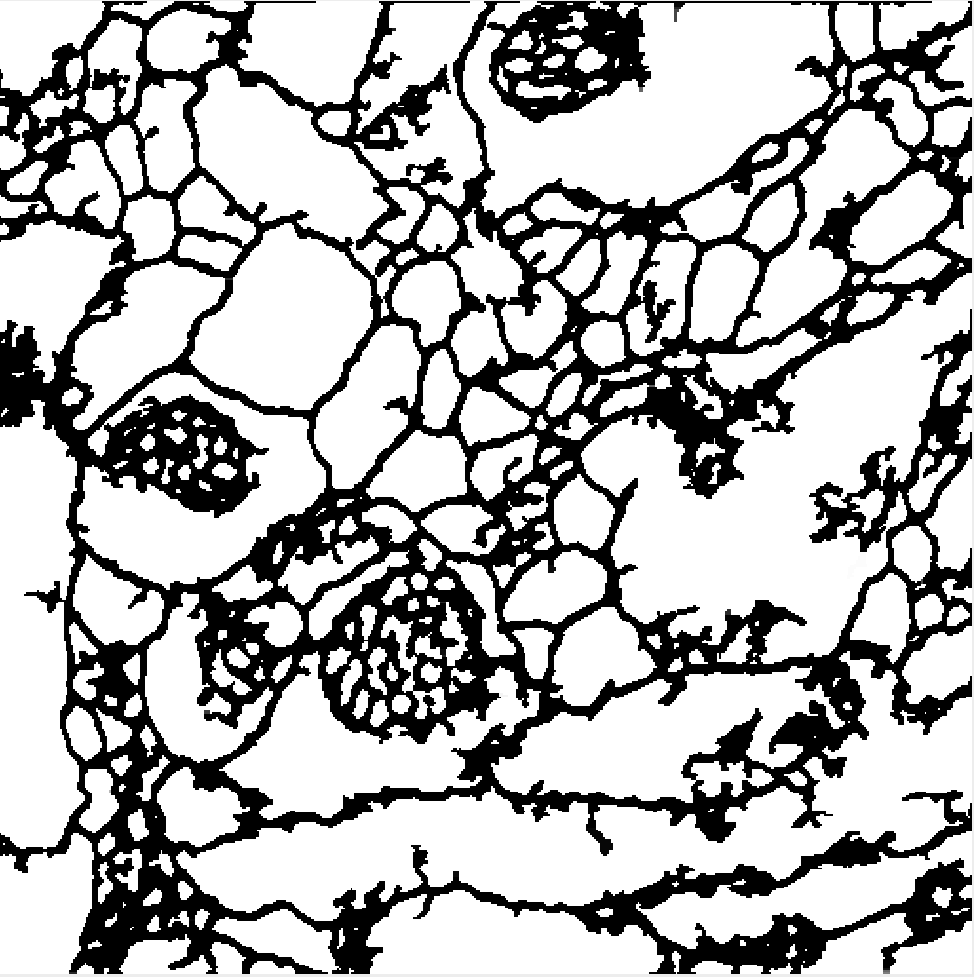
\includegraphics[height=0.7\textwidth]{./images/isbi_out_1.png}
        \caption{Our segmentation}
    \end{subfigure}
    \begin{subfigure}[t]{0.31\textwidth}
        \centering
        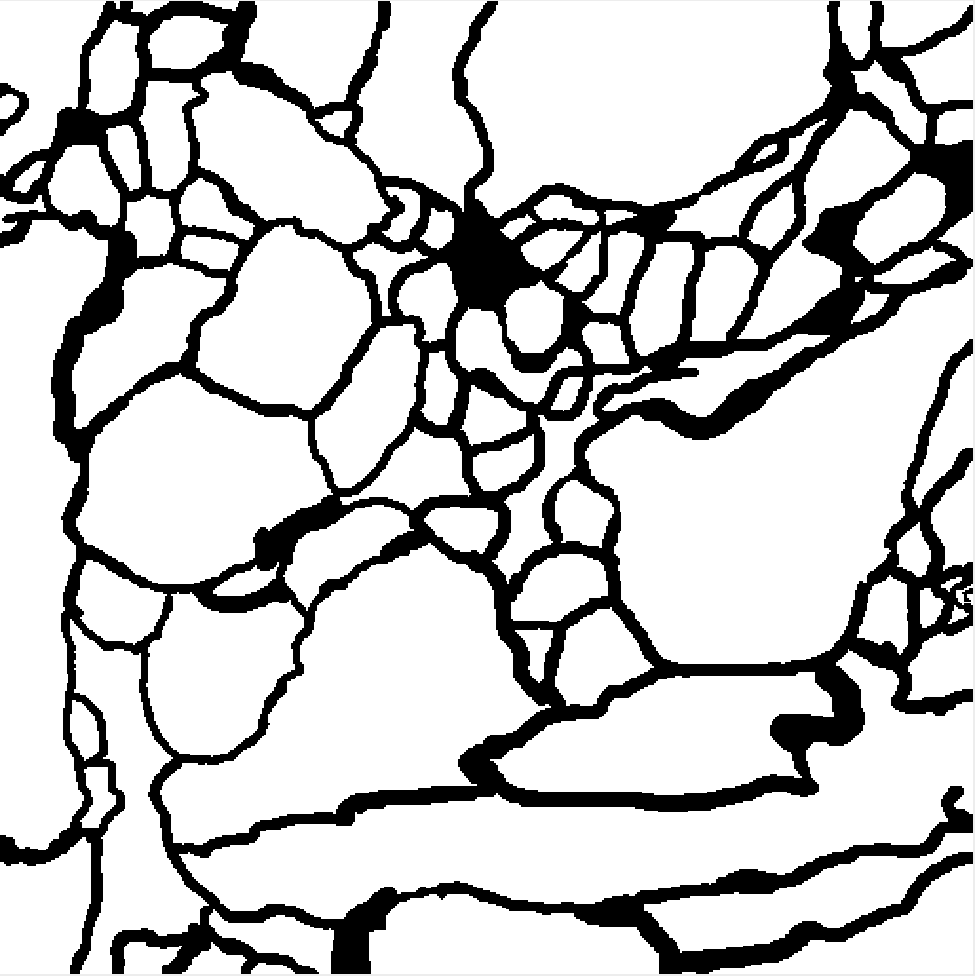
\includegraphics[height=0.7\textwidth]{./images/isbi_gt_1.png}
        \caption{Groundtruth}
    \end{subfigure}
	\caption{Results on the ISBI dataset (Training set)}
	\label{fig:isbi_result_train}
\end{figure}

As we can see in figure~\ref{fig:isbi_result_train} we are able to get a good
segmentation, with the same issue as before with the darker nuclei. We can also
see some "cracks" in our objects which was not an issue with the CREMI dataset.

\begin{figure}[!htbp]
    \centering
    \begin{subfigure}[t]{0.31\textwidth}
        \centering
        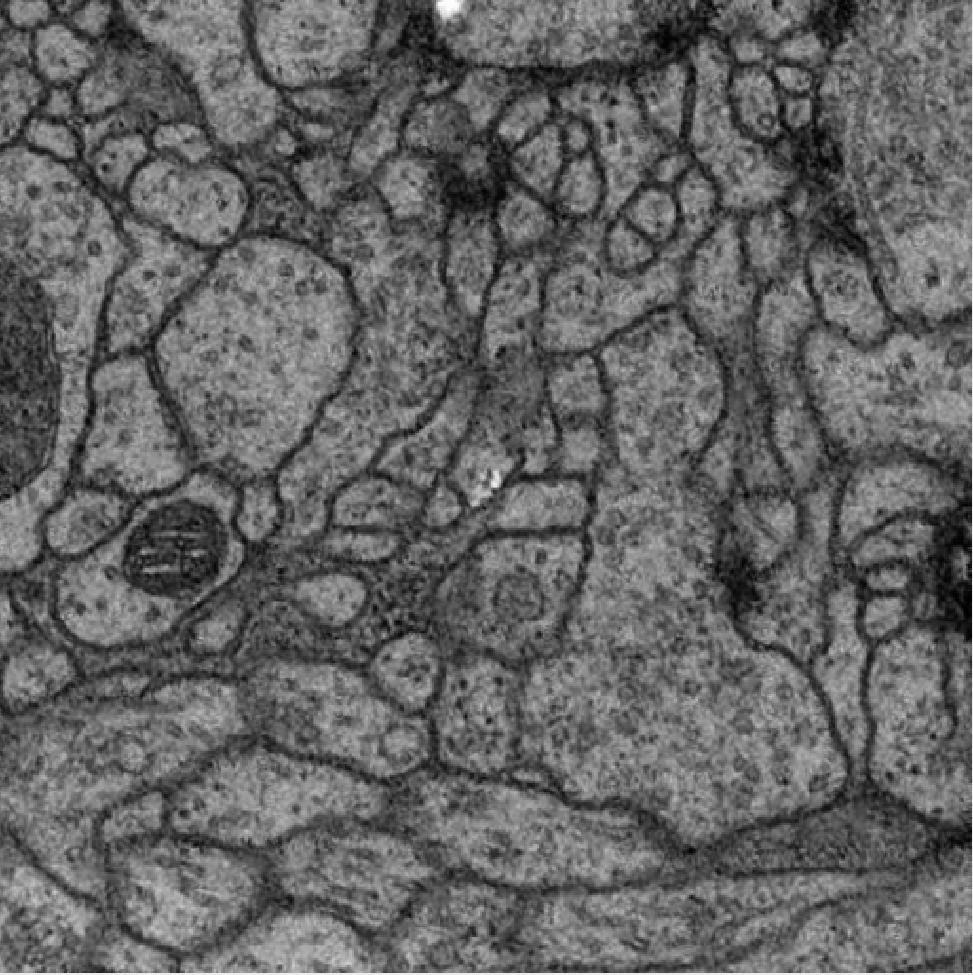
\includegraphics[height=0.7\textwidth]{./images/isbi_orig_2.png}
        \caption{Original image}
    \end{subfigure}%
    \begin{subfigure}[t]{0.31\textwidth}
        \centering
        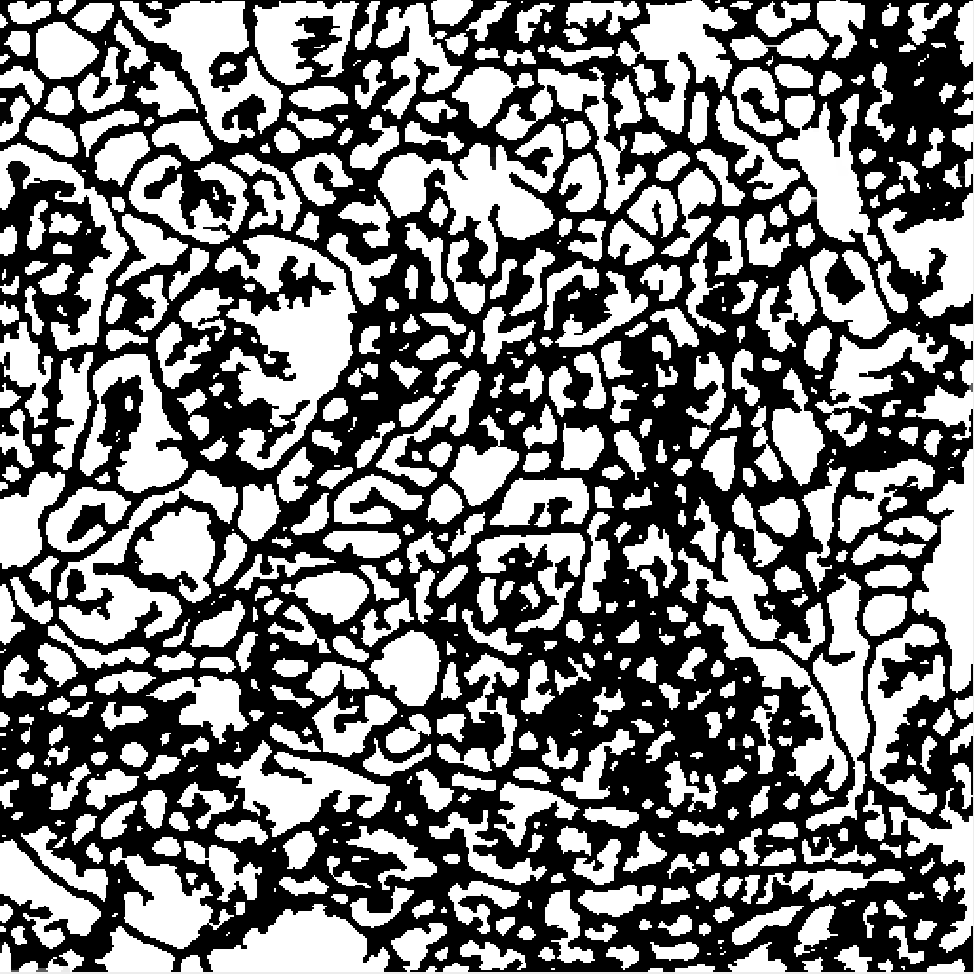
\includegraphics[height=0.7\textwidth]{./images/isbi_out_2.png}
        \caption{Our segmentation}
    \end{subfigure}
    \begin{subfigure}[t]{0.31\textwidth}
        \centering
        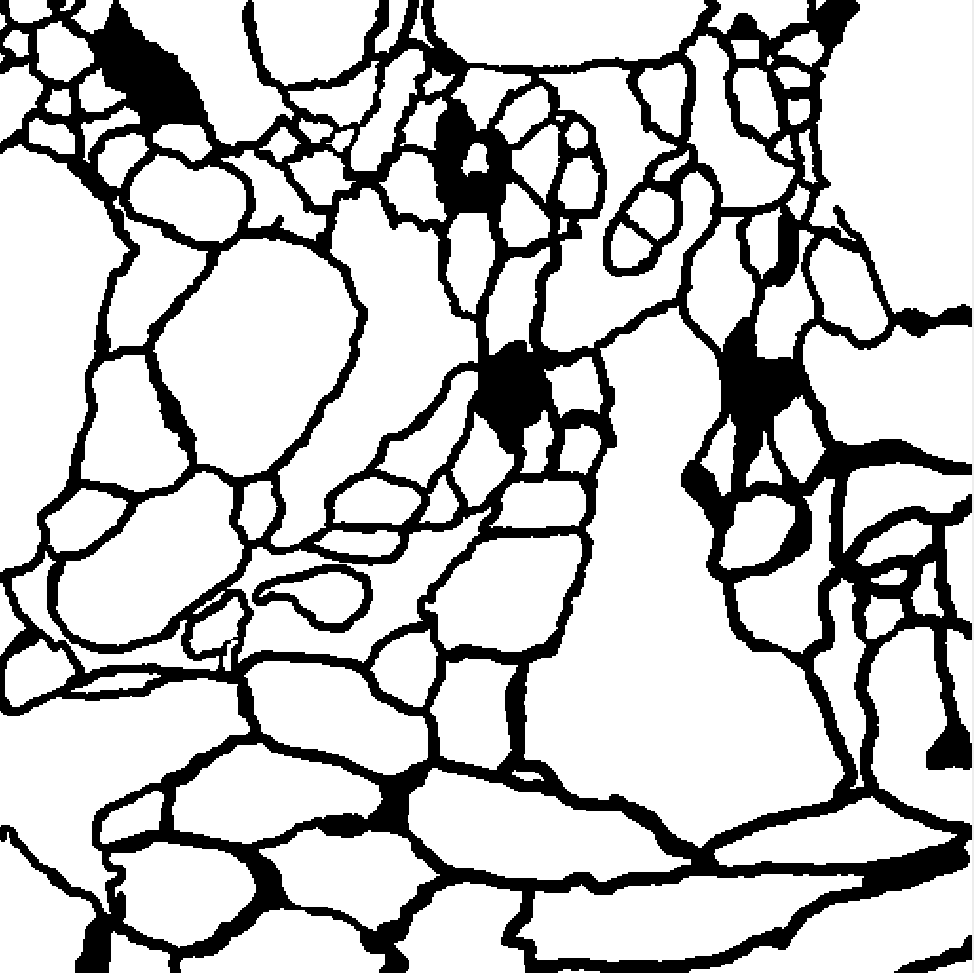
\includegraphics[height=0.7\textwidth]{./images/isbi_gt_2.png}
        \caption{Groundtruth}
    \end{subfigure}
	\caption{Results on a less constrasted image of the ISBI dataset (Training
	set)}
    \label{fig:isbi_result_fail}
\end{figure}

However the results are not always this good. As we can see in
figure~\ref{fig:isbi_result_fail}, we obtain a poor segmentation, where every
object is oversegmented and few borders are visible. This was the worst result
that we got.\\
This image is also the least constrasted, that's why we can hypotesize that the
oversegmentation issue comed from the lack of contrast of the image.\\

We evaluate through the same metrics as for the CREMI dataset, that is to say the Rand index and the VOI.
This time the VOI should be higher to be better.\\
We were not able to find exactly how the VOI was computed in both cases and
where the difference lies as to which values are obtained. More works need to
be put on understanding the computations of those metrics as to be able to
analyze them better.

\begin{table}[!htbp]
	\centering
	\begin{tabular}{|c|c|c|}
		\hline
		& Rand index & VOI \\
		\hline
		MALIS : Training set & 0.76 & 0.89\\
		\hline
		MALIS : Test set & 0.73 & 0.87\\
		\hline
		Thresholding : Test set & 0.752 & 0.82\\
		\hline
	\end{tabular}
	\caption{Results on the ISBI dataset}
	\label{tab:isbi_res}
\end{table}

As we can see in table~\ref{tab:isbi_res} the Rand index on our training set was 0.76 and 0.73 for the test test, 
which is similar but still higher than a thresholding which gets a Rand index of 0.72.
Our VOI is also a bit higher than the threshold.\\
Those are better results than CREMI's probably due to the small size of the
image and the thick borders in the output segmentation.\\ 

The results are also encouraging, as was to be expected since both datasets are
very similar.

